\chapter{Synthesis}
\label{Synthesis}
The synthesis of the design has been achieved by a script (see Appendix \ref{appendix11}) which contains also the proposed synthesis algorithms. In addition, the script is also in charge of adjusting the environment variables and folders needed for the synthesis and later for the physical design script.\\\\
The synthesis has been done through an inductive approach. As first step, a simple design without any constraints has been synthesized and evaluated. For moving inside the design space, the next step has been using as constrained on the clock different percentage values of the non-constrained synthesized design clock. Different percentage has been used, from 1\% up to 20\% (increase of clock frequency wrt to the non-constrained synthesized clock). Moreover, in this case as synthesis approach \textit{compile\_ultra} has been used for pushing more effort in general optimizations (compared with the non-constrained design, where only \textit{compile} has been used). The estimation of the area as much as possible to a real processor has been achieved by the usage of Scan Flip Flops instead of the normal Flip Flops (available in the used library).\\
As next degree of freedom, in the design space, all the previous designs with different clock constraints have been synthesized putting a constraint on finding the minimum area.

\section{Results}
The results in terms of area, latency and area are collected and presented as graphs.\\
As first design space, the latency-area graph can be seen in Figure \ref{fig:lat_area}:
\begin{figure}[!htbp]
\centering
\captionsetup{justification=centering}
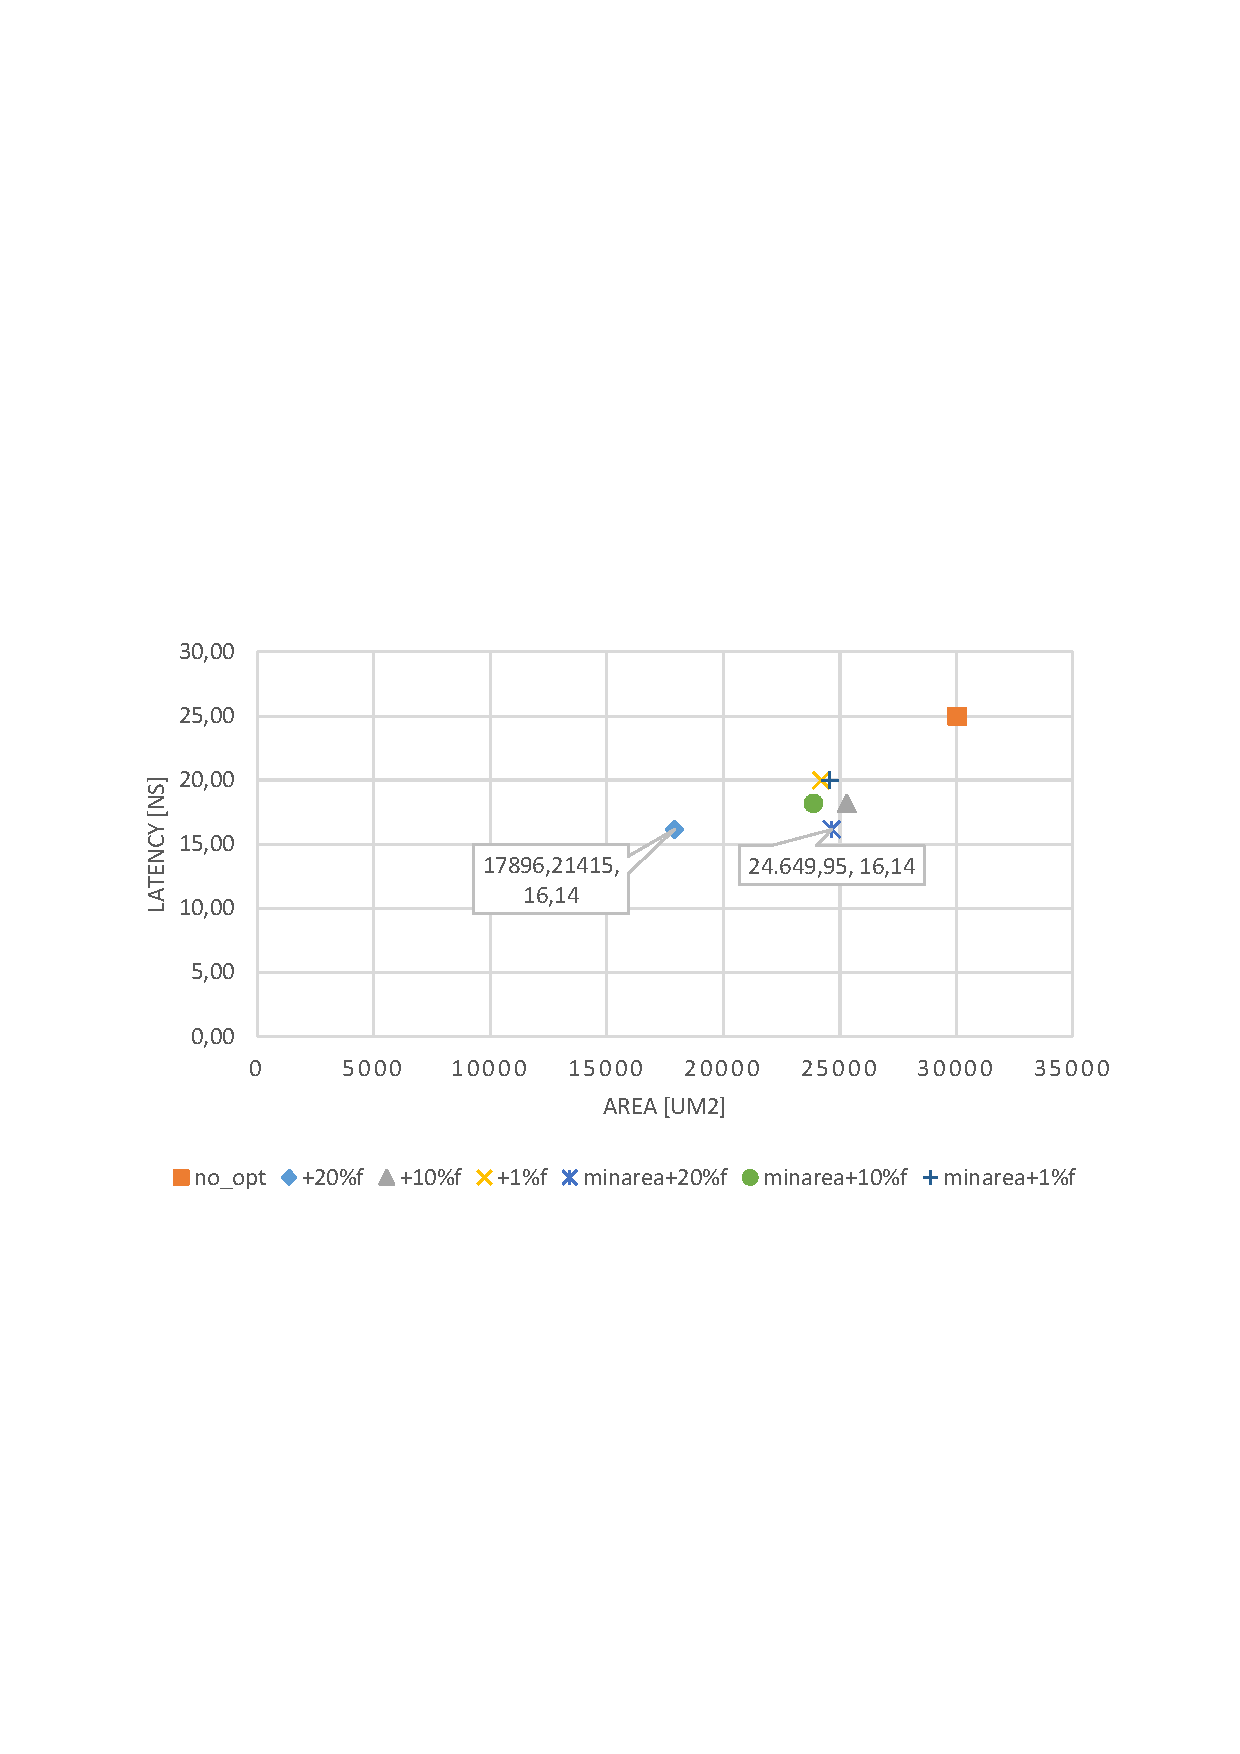
\includegraphics[scale=0.5,angle=0]{./chapters/files/latency_area.pdf}
\caption{Design space: Area \protect\footnotemark[1] vs Latency}
\label{fig:lat_area}
\end{figure}\\
\footnotetext[1]{Cell area}
In this design space, the best design is the one synthesized with a clock frequency greater than the 20\% of the non-constrained design frequency and without no constraints on the area.\\

Moreover, a further extension of the previous design space may be the power consumption (where also constrains can be added). In Figure \ref{fig:area_power_latency} it is presented the power consumption of the constraints on area and latency.
\begin{figure}[!htbp]
\centering
\captionsetup{justification=centering}
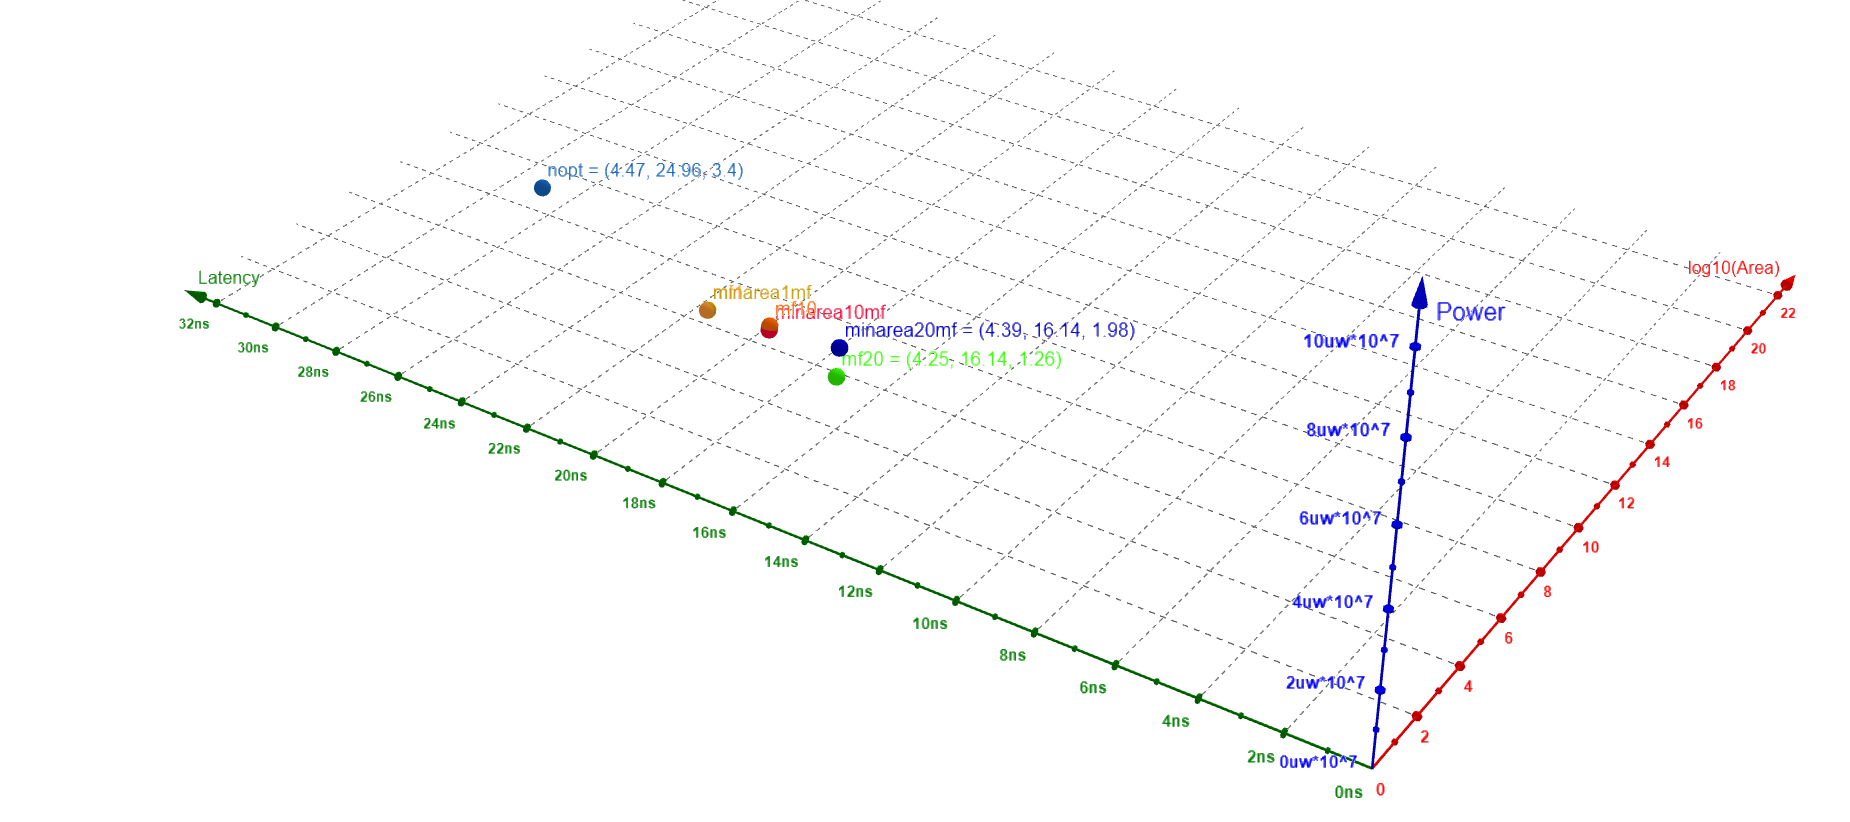
\includegraphics[scale=0.22,angle=0]{./chapters/files/latency_area_power.png}
\caption{Design space: Area vs Latency vs Power}
\label{fig:area_power_latency}
\end{figure}\\
An as best design, it is still the one synthesized with 20\% more of frequency. This result is probably due to the synthesis strategies and choices which lead to the best results of this design in terms of power, area and latency even with the only constraint on the latency. On the other hand, the design with constraint on minimum area results to have a bigger area compared with the one without the constraint, this may be the results of different optimization choices dictated from the presence of area constraints. \\\\

In the following table the results from synthesis reports are summarized:\\
\begin{table}[h!]
\centering
\begin{tabular}{ |p{3cm}||p{3cm}|p{3cm}|p{3cm}|  }
 \hline
Design & Area [\textmu $m^2$] & Latency [ns] & Power [\textmu W]\\
 \hline
 No optimization   &30034,85832	&24,96&	3,40E+07\\
  \hline
 + 20\% frequency & 17896,21415	&16,14	&1,26E+07\\
  \hline
 + 10\% frequency &25306,70806&	18,15&	1,87E+07\\
  \hline
 + 1\% frequency & 24199,08403	& 19,97	&1,69E+07\\
 \hline
 + 20\% frequency and minarea & 24649,95403	&16,14&	1,98E+07\\
  \hline
 + 10\% frequency and minarea&23870,84002	& 18,15&	1,78E+07\\ 
\hline
 + 1\% frequency and minarea& 24569,62203	& 19,97 &	1,69E+07\\
 \hline

\end{tabular}
\caption{Area-Latency-Power points in Design space}
\label{table:1}
\end{table}

